\begin{center}
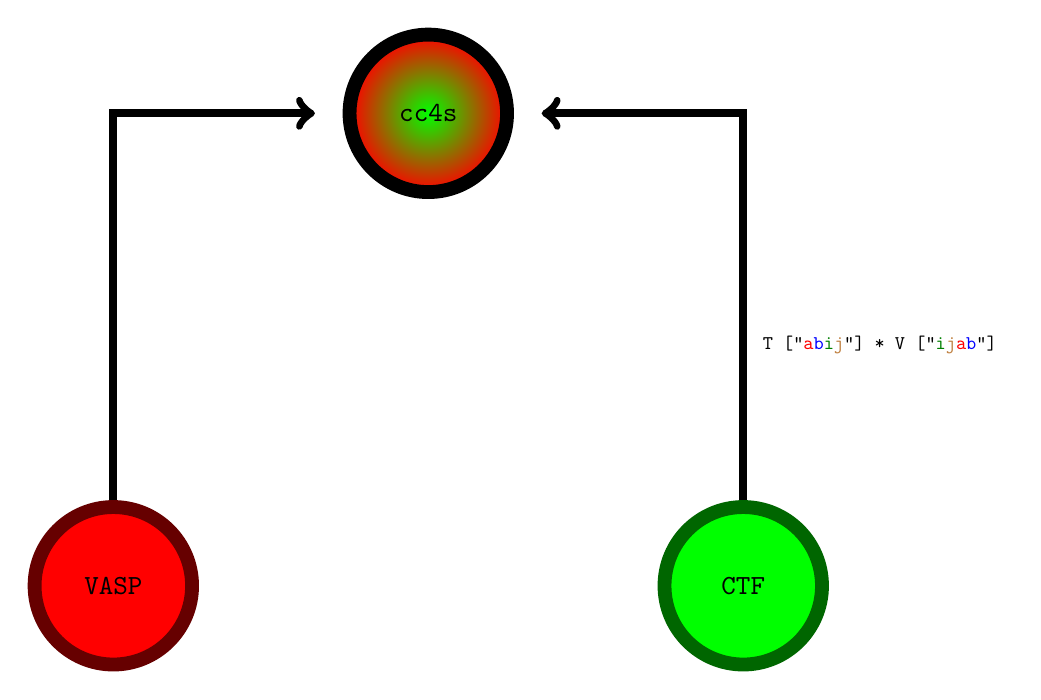
\begin{tikzpicture}[style={
    blob/.style={
      node distance=4cm,
      minimum size=2cm,
    },
    cc4sstyle/.style={
      blob, circle,
      line width=5,
      inner color=green,
      outer color=red,
      draw,
    },
    ctfstyle/.style={
      blob, circle,
      line width=5,
      fill=green,
      draw=green!40!black,
    },
    vaspstyle/.style={
      blob, circle,
      line width=5,
      fill=red,
      draw=red!40!black,
    },
    myarrow/.style={->, shorten >=10pt, line width=3pt}
  }]
  \draw[]
    node[cc4sstyle] (cc4s) {\texttt{cc4s}}
    node[vaspstyle, below of=cc4s, left of=cc4s, yshift=-2cm] (vasp) {
      \texttt{VASP}
    }
    node[pos=0.5] {
    }
    node[ctfstyle, below of=cc4s, right of=cc4s, yshift=-2cm] (ctf) {
      \texttt{CTF}
    }
  ;
  \draw[myarrow] (vasp.north) |- (cc4s.west);
  \draw[myarrow]
    (ctf.north) |- (cc4s.east)
    node[pos=0.2, scale=0.7, right] {
      \texttt{
        T
        ["{\color{red}a}{\color{blue}b}{\color{green!50!black}i}{\color{brown}j}"] *
        V
        ["{\color{green!50!black}i}{\color{brown}j}{\color{red}a}{\color{blue}b}"]
      }
    }
  ;
\end{tikzpicture}
\end{center}

%\begin{itemize}
  %\item
    %Implementation in package \texttt{cc4s} (\textit{Coupled Cluster for
    %solids})
  %\item DFT and HF calculations performed with \texttt{VASP}
  %\item Plane waves basis set
  %\item Cyclops tensor framework (\texttt{CTF}) as a tensor contraction engine
%\end{itemize}
